\documentclass[tikz,border=2]{standalone}
\usetikzlibrary{shadows,arrows,shapes,positioning,calc,backgrounds,fit}
% Define the layers to draw the diagram
%
\begin{document}
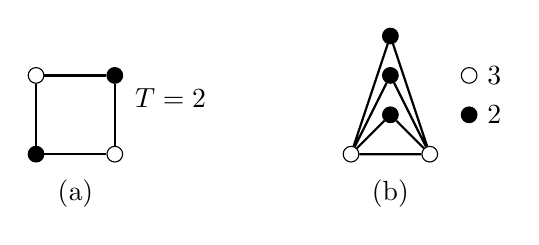
\begin{tikzpicture}
[node distance=1cm,
vertex/.style={shape=circle,draw=black,inner sep=2pt},
myedge/.style={thick}]
%%
\node (v1) [vertex,fill] at (0,0) {};
\node (v2) [vertex,right of=v1] {};
\node (v3) [vertex,fill,above of=v2] {};
\node (v4) [vertex,above of=v1] {};
\draw[myedge] (v1) -- (v2) -- (v3) -- (v4) -- (v1);
%% \draw[myedge,dashed] (v2) -- (v4);
\node [above right of=v2] {$T=2$};
\node at (0.5,-.5) {(a)};
%%

\node (v1) [vertex] at (4,0) {};
\node (v2) [vertex,right of= v1] {};
\node (v3) [vertex,fill] at (4.5,.5) {};
\node (v4) [vertex,fill] at (4.5,1) {};
\node (v5) [vertex,fill] at (4.5,1.5) {};
\draw[myedge] (v1) -- (v2) -- (v3) -- (v1) -- (v4) -- (v2) -- (v5) -- (v1);
\node (a) [vertex,fill,label=right:$2$] at (5.5,0.5) {};
\node (b) [vertex,label=right:$3$] at (5.5,1) {};
\node at (4.5,-.5) {(b)};
\end{tikzpicture}
{}
\end{document}
